\documentclass[letterpaper,12pt,leqno]{article}
\usepackage{paper}
\usepackage{pdflscape}
\bibliographystyle{bibliography}

% Enter paper title:
\hypersetup{pdftitle={Improving Rural Accessibility in Indonesia: Fuel Subsidy versus Infrastructure Development}}

% Enter permanent URL to paper
\codeavailable{https://github.com/maghfiraer/ECON7023-Metrics-II/tree/main/Final_Project}

% Enter BibTeX file with references:
\newcommand{\bib}{bibliography.bib}

% Enter PDF file with figures here:
\newcommand{\pdf}{figures.pdf}

% Custom math
\newcommand\iid{\stackrel{\mathclap{iid}}{\sim}}
\newcommand\asym{\stackrel{\mathclap{a}}{\sim}}
\newcommand\convprob{\xrightarrow{p}}
\newcommand\convdist{\xrightarrow{d}}
\newcommand{\N}{\mathbb{N}}
\newcommand{\Z}{\mathbb{Z}}
\newcommand{\E}{\text{E}}
\newcommand{\V}{\text{Var}}
\newcommand{\Av}{\text{Avar}}
\newcommand{\se}{\text{se}}
\newcommand{\corr}{\text{Corr}}
\newcommand{\cov}{\text{Cov}}
\newcommand{\norm}{\text{Normal}}
\newcommand{\indep}{\perp \!\!\! \perp}
\newcommand{\Hy}{\text{H}}

% Fill out paper:
\begin{document}
\title{Improving Rural Accessibility in Indonesia: Fuel Subsidy versus Infrastructure Development}
\author{Maghfira Ramadhani
\thanks{Maghfira Ramadhani: Ph.D. student at Georgia Institute of Technology, maghfira.ramadhani@gatech.edu}}
\date{April 2023}                       
\begin{titlepage}\maketitle

Indonesia has been subsidizing transportation costs for a long time.

\end{titlepage}\section{Introduction}\label{s:introduction}
 
\paragraph{Research question} Although Indonesia has been subsidizing fuel for a long time, high fuel prices were still observed in rural areas in the last decade since they were unable to get the fuel from the official fuel supply chain \citep{liputan_2016, jawapos_2017}. Therefore since 2016, the government initiated the One Price Fuel program to guarantee the availability of subsidized fuel in these areas. The government in collaboration with the National Oil Company started to build a new gas station in the targeted outermost and less-developed village so that they get the fuel at the same price as any other gas station. This program is expected to bring development to the village level by reducing energy costs which could improve the overall village's economic activity. On the other hand, decentralization of development to the village level has been implemented since 2014, when the central government initiate an annual fiscal transfer to the village government to improve their financial capability in bringing development to the last miles\footnote{See Village Law No. 6 of 2014}. This research measures the impact of these government programs in improving rural accessibility at the village level and exercising the efficiency of each specific program.

\paragraph{Answer to the question} In addressing the research question, this research uses unit transportation cost to measure accessibility. Specifically in rural areas, \citet{sambodo_2019} find that transportation spending dominates energy spending which could limit people's mobility and slow economic development. On the other hand, the lack of adequate and reliable infrastructure drives up the transportation cost \citep{sandee_2016}. I treat the unit transportation cost as the willingness to pay for transportation in rural areas, therefore we control for other factors affecting the demand structure to get the causal effect. I use panel data analysis to measure the impact of the two programs in improving rural accessibility. Regarding the fuel program, I obtain the list of 55 government-appointed new distributor locations from the National Oil Company (NOC). I use the village fund transferred to the village government as a proxy for village infrastructure development. From a political economy perspective, infrastructure development is managed by the government directly, while the fuel subsidy is managed through the National Oil Company (NOC) as a delivery agent \citep{ichsan_2022}. This research evaluates the efficiency of the program by comparing the reduction of transportation cost per budget spent as the benefit-cost ratio.

\paragraph{Related literature} This paper builds on the literature on rural development and fossil fuel subsidy in Indonesia. Related literature has indicated that both subsidizing fuel and inter-government transfer contributed to improving the general economic condition in rural areas \citep{sambodo_2019,ichsan_2021,hartojo_2022}. \citep{sambodo_2019} find that villages with better access to energy tend to divert away their spending more productively thus having better health outcomes. \citep{ichsan_2021} argued that the fuel program is a short-term remedy for reducing transportation costs in rural areas, and believes that infrastructure development is the sustainable way to do so. On the effect of village fund transfer, \citet{hartojo_2022} show that the transfer effectively improved rural economic growth in rural areas. This research is the first to evaluate and compare the impact of both programs in improving accessibility at the village level.

\paragraph{Outline} The rest of the paper is organized as follows. I develop the institutional context and conceptual framework for the discussion in Section \ref{s:framework}. Section \ref{s:data} describes the data and its summary statistics. Section \ref{s:result} discusses the findings and provides a robustness check and evaluates the benefit-cost of the programs. Section \ref{s:conclusion} provides a concluding remark of the discussion.

\section{Institutional Context and Conceptual framework}\label{s:framework}

In this section, I discussed the institutional context of Indonesia and build a conceptual framework for understanding the impact of how the fossil fuel program and village development can improve rural accessibility.

\subsection{Accessibility in rural area}

\paragraph{Accessibility challenge in Indonesia}
Following \citet{sandee_2016}, regarding rural accessibility in Indonesia, the challenge mainly related to intra-island connectivity ---links within individual islands--- is linking underdeveloped regions to growth centers. In the densely populated part of Java island, the city is the center of growth, the challenges of connectivity are mostly congestion-based challenges causing high-cost for mobility. In contrast, in the rural areas of Java, we can still find a village that we can only access by motorcycle or even only by foot. This challenge is somewhat similar in other main islands such as Sumatra, Kalimantan, Sulawesi, and Papua. In these other mainlands, the challenges are the existence of adequate and reliable infrastructure that drives up transportation costs. The government initiatives in attracting foreign capital and facilitating public-private partnerships in bringing a large-scale infrastructure development have been a policy priority since 2015 \citep{pwc_2016}.


\paragraph{Transportation cost as a measure of accessibility} We can treat unit transportation cost as the willingness to pay or demand for transportation. We follow previous literature on willingness to pay for rural transportation from revealed preference, the affecting factors include travel time, convenience, and trip purpose i.e. work or education.



\subsection{Fossil fuel subsidy regime}

Indonesia used to be a large oil exporter in the oil boom period in the 1970s and 1980s and the National Oil Company (NOC), Pertamina contributed a big part in delivering the fuel subsidy to the public \citep{ichsan_2022}. However, as the production declined, there has been increased pressure for subsidy reform. 

\subsection{Decentralization of development}

Developing countries believe decentralization and local government reform are more efficient in bringing local development \citep{vazquez_2017} and providing public goods better than central government \citep{arends2020}. In 2014 the government enacted village fund transfer to implement decentralization at the village level. The allocation amount takes into account village conditions, i.e. poverty and geographic difficulty into account.

\section{Data}\label{s:data}

\paragraph{Data source} I obtained the Village Potential Statistics data for the years 2014 and 2018 from Indonesia's Central Bureau of Statistics complemented with village fund transfer data from the Ministry of Village Development. The original survey covers general information about the village, population and employment, housing and environment, natural disaster, education and health, sport and leisure, transportation and communication, land use, economic activity, security, local government, community empowerment, and agriculture. However, not all the variables are published due to potential inaccuracy issues. The original data consists of consecutively 82,190 and 83,931 observations of villages in rural and urban areas. The data is then cleaned to only include non-urban areas.

\paragraph{Data description} Natural disaster data reported are up to three years before the survey, but I only use the data on landfall and earthquake occurrence from the previous year as it represents the most recent physical condition of the village from the years 2014 and 2018. Geographic data available are binary variables about mainland topography, location relative to the sea, location relative to the forest, and the use of rivers for transportation. The mainland topography variable is equal to 1 if the village is located on a slope or valley and equal to 0 if it is located on a vast land. The binary variable on sea relative location is equal to 1 if the village has a border with the sea, and equal to 0 if otherwise. Similarly, the binary variable on forest relative location is equal to 1 if the village is inside or has a border with the forest, and equal to 0 if otherwise. The river transportation binary variable with the value of 1 indicates that the river is used for transportation in the village.

Regarding infrastructure status, data on education infrastructure and electrification are available. The data on education infrastructure range from the number of schools from elementary to university in the area. However, we only use the number of Junior High Schools and Senior High Schools data as people usually require daily travel for this level of education, thus will affect the demand for transportation. For elementary education, parents are more likely to send their children to the one closest to their village. While for university besides it is usually unavailable at the village level, students usually migrate and move out of their parent's house to live close to the university. I use the number of electricity customer households from the National Electricity Company (PLN).

Regarding the village's economic condition, the only available data from the survey is the number poverty letter statement released by the village government for the year. Other demographic data are not available in the survey. These data are usually available only at the district or sub-district level at the lowest administrative level. In this research, I use the number of poverty letter statements as a proxy for the economic condition of the village.

A variety of data on transportation are available including travel duration (in hours), travel distance (in kilometers), and travel cost (in thousand Rp.). All the variables are measured from the village office to the sub-district office, the district office, the other sub-district office closest to the village, and the other district office closest to the village. For this analysis, I only use the variable measure from the village office to the sub-district office.

I measure rural accessibility using the unit transportation cost (in Rp/km) of each individual village $i$ for the year $t$. I define unit transportation cost, $y_{it}$, as the transportation cost from the village $i$'s office to the sub-district office (in thousands Rp) at year $t$, $c_{it}$, divided by the distance from the village office $i$'s to the sub-district office (in km) at year $t$, $d_{it}$ as shown in equation \eqref{e:1}.
\begin{equation}
        y_{it}=c_{it}/d_{it}\label{e:1}
\end{equation}

I obtain the list of 55 government-appointed new distributor village locations that were built in 2016 and 2017 from the NOC. Figure \ref{f:3} show the detailed map of these locations. define all the villages that are in the same sub-district as treated by the program, i.e. $D_{it}=1$ in the year 2018. Note that in the year 2014, all villages have $D_{it}=0$. For example, suppose the government in 2016 gives the order for the NOC to build a new distribution point at village $A$. Village $A$ is in the same sub-district as villages $B,C$, and $D$. Then all villages $A,B,C$, and $D$ are treated. To extend the discussion, I use two different samples at the province level and the district level. The other main explanatory variable is the village fund transfer measured in millions Rp.

The summary statistics of the variables are presented in Table \ref{t:1} and Table \ref{t:2}. As seen in both tables, the  unit transportation cost is on average lower in 2018 than in 2014. Also the village fund transfer on average increased in 2018 than in 2014.


\section{Empirical strategy}\label{s:strategy}

I follow the following model specification
\begin{equation}
    y_{it}=\alpha_i+\theta_t+\delta_1 D_{it}+\gamma_1 VF_{it}+\textbf{X}\pmb{\beta}+\varepsilon_{it}\label{e:2}
\end{equation}
where $y_{it}$ represents the unit transportation cost in village $i$ in year $t$,
$\alpha_i$ represents the village fixed effects, $\theta_t$ represents time trend or time fixed effects, $D_{it}$ and $VF_{it}$ is the main variable of interests, and $\textbf{X}$ as vector of covariates affecting demand. In equation \eqref{e:2}, the impact of the fuel program on the transport cost is given by the coefficient $\delta_1$, while the impact of the village fund transfer. Serial correlation should not be an issue in this model since the panel is 4 years apart. 

I perform \citet{hausman78} specification test. The test of $H_0:$ difference in coefficients not systematic or the individual unobserved heterogeneity is correlated with the regressors. We can compute the Hausman statistic as \begin{equation*}
        H=(\hat{\pmb{\delta}}_{FE}-\hat{\pmb{\delta}}_{RE})'\left[\hat{\Av}(\hat{\pmb{\delta}}_{FE})-\hat{\Av}(\hat{\pmb{\delta}}_{RE})\right]^{-1}(\hat{\pmb{\delta}}_{FE}-\hat{\pmb{\delta}}_{RE}) \asym \chi_M^2 \end{equation*}
The test yields a $\chi^2$-statistics of 15.96 with $P$-value of 0.0003, thus we cannot reject the null hypothesis. This suggests using fixed effects instead of random effects for panel data analysis. This test is valid under RE1-RE3, thus we can not strictly argue with it.

Possible endogeneity treats from Village Fund Transfer $(VF_{it})$ and Treatment $(D_{it})$, therefore I need to identify whether there is a good instrument available in the dataset. If the two main variables are endogenous, \al{Fixed Effect Instrumental Variable} (FEIV) approach (similar to FDIV for $T=2$) can be applied to identify $\delta_1$ and $\gamma_1$ in equation \eqref{e1}.

\section{Results}\label{s:result}
\subsection{Main findings}

\paragraph{Findings 1}
        Panel OLS estimates indicates that \al{only the fuel program significantly affected unit transportation costs} in rural areas when using the \al{province as sample}, and \alg{both program significantly affects unit transportation cost} when using the \alg{district as sample}. 
        
\paragraph{Findings 2}
        FEIV estimates yield insignificant estimates. Endogeneity tests against $H_0$ that village fund transfer and fuel program are exogenous yield a $P$-value of consecutively 0.9103 and 0.5125, indicating that \al{the null hypothesis can not be rejected}. It might be \alg{better to use Panel OLS} instead.

\paragraph{Findings 3}
        I enrich the analysis by generating an interaction variable between programs to explore the complementary effect of both programs. The interaction term is \al{statistically insignificant}.

\subsection{Benefit-cost analysis}
The village fund transfer reduces unit transport cost by \al{1 Rp/km} per millions Rp spent. The fuel program reduces unit transport costs by \al{2,380 Rp/km} per gas station built. The capital cost of building one remote gas station is reported to be around 3 billion Rp and the profit margin of sales is 195 Rp/Liter\footnote{See \href{https://www.cnbcindonesia.com/news/20201213090547-4-208715/bangun-spbu-bbm-satu-harga-ternyata-lama-balik-modalnya}{https://www.cnbcindonesia.com/news/20201213090547-4-208715/bangun-spbu-bbm-satu-harga-ternyata-lama-balik-modalnya}} and average total sales per location of 383 kL\footnote{The figures is obtained from Indonesian Downstream Oil and Gas Authority} in the 2016-2017 period.
Thus we can estimate the benefit/net cost of the fuel program as
\begin{align*}
   \left. B/C&=\frac{2,380 \text{ Rp/km}}{\text{location}}\middle/\underbrace{\frac{3,000 \text{ million Rp}-\frac{195\text{ Rp}}{kL}\times 383\text{ kL}\times\frac{\text{ million Rp}}{10^6\text{ Rp}}}{\text{location}}}_{\displaystyle \text{Net Cost} = \text{Capital Cost} - \text{Sales Profit}} \right.\\
   &=0.79\ \frac{\text{Rp/km}}{\text{millions Rp spent}}.
\end{align*}
Village fund transfer \alg{is more efficient} than the fuel program in increasing rural accessibility.

\section{Conclusion}\label{s:conclusion}

This research finds out that both rural fuel distribution program and inter-government transfer significantly reduces unit transportation cost in rural areas. 

The village fund transfer successfully reduces unit transport cost by 1 Rp/km per million Rp spent, while the fuel program reduces unit transport cost by 0.79 Rp/km per million Rp spent. This indicates that the fund transfer to local government is more efficient in improving rural accessibility.

\paragraph{Further recommendation}
The limited nature of the data really limits the analysis in this paper, thus I suggest collecting more data by adding one more year of observation to be able to implement a more robust analysis on time-varying variation.

Following \citet{abadie2016}, I suggest implementing Propensity Score Matching to construct an artificial control group by matching each treated unit with a non-treated unit of similar characteristics.

\bibliography{\bib}

% Fill out appendix:
\newpage
\appendix
\begin{landscape}
\section{Tables}\label{a:table}

\begin{table}[h]
\caption{Summary statistics of variables with the province-level as sample} 
\scalebox{0.85}{\begin{tabular}{l*{2}{ccccc}}
\toprule
                &     2014&         &         &         &         &     2018&         &         &         &         \\
                &     Mean&     S.D.&      Min&      Max&     Obs.&     Mean&     S.D.&      Min&      Max&     Obs.\\
\midrule
\emph{Transportation}&         &         &         &         &         &         &         &         &         &         \\
\hspace{0.25cm} Unit transportation cost in 000s Rp./km&     3.29&    19.94&     0.00&  1000.00&    38624&     3.22&     9.36&     0.00&   800.00&    38646\\
\hspace{0.25cm} Travel duration (hrs)&     1.17&     1.44&     1.00&    99.00&    38624&     0.50&     1.41&     0.00&    60.50&    38646\\
\\ \emph{Natural Disaster}&         &         &         &         &         &         &         &         &         &         \\
\hspace{0.25cm} Landfall occurence average per year&     0.11&     0.52&     0.00&     9.00&    38624&     0.15&     0.62&     0.00&     9.00&    38646\\
\hspace{0.25cm} Earthquake occurence average per year&     0.04&     0.29&     0.00&     9.00&    38624&     0.23&     1.07&     0.00&     9.00&    38646\\
\\ \emph{Infrastructure}&         &         &         &         &         &         &         &         &         &         \\
\hspace{0.25cm} Number of PLN electricity user household&   656.51&   781.91&     0.00& 14460.00&    38624&   738.27&   887.98&     0.00& 17530.00&    38646\\
\hspace{0.25cm} Number of Junior High School&     0.53&     0.82&     0.00&    14.00&    38624&     0.58&     0.86&     0.00&    12.00&    38646\\
\hspace{0.25cm} Number of Senior High School&     0.26&     0.70&     0.00&    40.00&    38624&     0.31&     0.74&     0.00&    11.00&    38646\\
\\ \emph{Geographic condition}&         &         &         &         &         &         &         &         &         &         \\
\hspace{0.25cm} =1 if slope/valleys, =0 vast land&     0.25&     0.43&     0.00&     1.00&    38624&     0.22&     0.41&     0.00&     1.00&    38646\\
\hspace{0.25cm} =1 if border with sea, =0 no border with sea&     0.19&     0.39&     0.00&     1.00&    38624&     0.19&     0.39&     0.00&     1.00&    38646\\
\hspace{0.25cm} =1 if inside or border with forest, =0 outside forest&     0.31&     0.46&     0.00&     1.00&    38624&     0.28&     0.45&     0.00&     1.00&    38646\\
\hspace{0.25cm} =1 if river used for transportation, =0 otherwise&     0.09&     0.28&     0.00&     1.00&    38624&     0.08&     0.27&     0.00&     1.00&    38646\\
\\ \emph{Economic condition}&         &         &         &         &         &         &         &         &         &         \\
\hspace{0.25cm} Number of poverty statement request&    73.52&   155.02&     0.00& 13705.00&    38624&    80.54&   327.46&     0.00& 10101.00&    38646\\
\\ \emph{Inter-government Transfer}&         &         &         &         &         &         &         &         &         &         \\
\hspace{0.25cm} Revenue from village fund transfer&   116.08&   213.26&     0.00&  7716.00&    38624&   121.07&   143.42&     0.00& 13662.00&    36630\\
\bottomrule
\end{tabular}
}
\note{The sample is all the villages in the provinces where the fuel program exists.}
\label{t:1}\end{table}


\begin{table}[h]
\caption{Summary statistics of variables with the district-level as sample} 
\scalebox{0.85}{\begin{tabular}{l*{2}{ccccc}}
\toprule
                &     2014&         &         &         &         &     2018&         &         &         &         \\
                &     Mean&     S.D.&      Min&      Max&     Obs.&     Mean&     S.D.&      Min&      Max&     Obs.\\
\midrule
\emph{Transportation}&         &         &         &         &         &         &         &         &         &         \\
\hspace{0.25cm} Unit transportation cost in 000s Rp./km&     5.14&    21.02&     0.00&  1000.00&     3407&     4.93&    12.47&     0.00&   400.00&     3411\\
\hspace{0.25cm} Travel duration (hrs)&     1.27&     1.27&     1.00&    30.00&     3407&     0.74&     2.36&     0.00&    60.50&     3411\\
\emph{Natural Disaster}&         &         &         &         &         &         &         &         &         &         \\
\hspace{0.25cm} Landfall occurence average per year&     0.07&     0.37&     0.00&     6.00&     3407&     0.10&     0.49&     0.00&     9.00&     3411\\
\hspace{0.25cm} Earthquake occurence average per year&     0.04&     0.35&     0.00&     7.00&     3407&     0.46&     1.60&     0.00&     9.00&     3411\\
\emph{Infrastructure}&         &         &         &         &         &         &         &         &         &         \\
\hspace{0.25cm} Number of PLN electricity user household&   366.92&   610.20&     0.00&  6726.00&     3407&   422.79&   651.77&     0.00&  6468.00&     3411\\
\hspace{0.25cm} Number of Junior High School&     0.54&     0.85&     0.00&     9.00&     3407&     0.61&     0.89&     0.00&    12.00&     3411\\
\hspace{0.25cm} Number of Senior High School&     0.27&     0.66&     0.00&     7.00&     3407&     0.33&     0.73&     0.00&     8.00&     3411\\
\emph{Geographic condition}&         &         &         &         &         &         &         &         &         &         \\
\hspace{0.25cm} =1 if slope/valleys, =0 vast land&     0.22&     0.42&     0.00&     1.00&     3407&     0.19&     0.39&     0.00&     1.00&     3411\\
\hspace{0.25cm} =1 if border with sea, =0 no border with sea&     0.41&     0.49&     0.00&     1.00&     3407&     0.41&     0.49&     0.00&     1.00&     3411\\
\hspace{0.25cm} =1 if inside or border with forest, =0 outside forest&     0.37&     0.48&     0.00&     1.00&     3407&     0.35&     0.48&     0.00&     1.00&     3411\\
\hspace{0.25cm} =1 if river used for transportation, =0 otherwise&     0.17&     0.37&     0.00&     1.00&     3407&     0.17&     0.38&     0.00&     1.00&     3411\\
\emph{Economic condition}&         &         &         &         &         &         &         &         &         &         \\
\hspace{0.25cm} Number of poverty statement request&    59.08&   141.93&     0.00&  4106.00&     3407&    69.00&   282.43&     0.00&  9999.00&     3411\\
\emph{Inter-government Transfer}&         &         &         &         &         &         &         &         &         &         \\
\hspace{0.25cm} Revenue from village fund transfer&   113.55&   129.92&     0.00&  1253.00&     3407&   158.93&   289.35&     0.00& 13662.00&     3172\\
\bottomrule
\end{tabular}
}
\note{The sample is all the villages in the districts where the fuel program exists.}
\label{t:2}\end{table}

\begin{table}[h]
\caption{Panel OLS estimates} 
\scalebox{0.85}{{
\def\sym#1{\ifmmode^{#1}\else\(^{#1}\)\fi}
\begin{tabular}{l*{4}{D{.}{.}{-1}}}
\toprule
                &\multicolumn{1}{c}{(1)}         &\multicolumn{1}{c}{(2)}         &\multicolumn{1}{c}{(3)}         &\multicolumn{1}{c}{(4)}         \\
\midrule
Treatment       &   -2.204\sym{*}  &   -2.173\sym{*}  &   -2.321\sym{**} &   -2.430\sym{**} \\
                &  (1.146)         &  (1.147)         &  (1.176)         &  (1.178)         \\
\addlinespace
Village Fund transfer&    0.000         &    0.000         &   -0.001\sym{*}  &   -0.001\sym{*}  \\
                &  (0.000)         &  (0.000)         &  (0.001)         &  (0.001)         \\
\addlinespace
Time trend      &   -0.086         &   -0.072         &    0.243         &    0.306         \\
                &  (0.113)         &  (0.111)         &  (0.306)         &  (0.284)         \\
\midrule
Observations    &    75254         &    75254         &     6579         &     6579         \\
\(R^{2}\)       &    0.000         &    0.000         &    0.008         &    0.003         \\
Adjusted \(R^{2}\)&    0.000         &    0.000         &    0.006         &    0.002         \\
Sample          & Province         & Province         & District         & District         \\
Controls        &      Yes         &       No         &      Yes         &       No         \\
Time Fixed Effects&      Yes         &      Yes         &      Yes         &      Yes         \\
Village Fixed Effects&      Yes         &      Yes         &      Yes         &      Yes         \\
\bottomrule
\multicolumn{5}{l}{\footnotesize Standard errors in parentheses}\\
\multicolumn{5}{l}{\footnotesize \sym{*} \(p<0.10\), \sym{**} \(p<0.05\), \sym{***} \(p<0.01\)}\\
\end{tabular}
}
}
\note{The sample is all the villages in the districts where the fuel program exists.}
\label{t:pols}\end{table}

\begin{table}[h]
\caption{FEIV Result with $D_{it}$ and $VF_{it}$ as endogenours }
\scalebox{0.8}{{
\def\sym#1{\ifmmode^{#1}\else\(^{#1}\)\fi}
\begin{tabular}{l*{8}{D{.}{.}{-1}}}
\toprule
                &\multicolumn{1}{c}{(1)}         &\multicolumn{1}{c}{(2)}         &\multicolumn{1}{c}{(3)}         &\multicolumn{1}{c}{(4)}         &\multicolumn{1}{c}{(5)}         &\multicolumn{1}{c}{(6)}         &\multicolumn{1}{c}{(7)}         &\multicolumn{1}{c}{(8)}         \\
\midrule
Treatment       &   18.297         & -132.775         &   16.617         & -135.896         &    3.825         &  -18.464         &    5.232         &  -19.610         \\
                & (14.523)         &(198.007)         & (13.596)         &(206.572)         &  (6.469)         & (28.313)         &  (6.040)         & (25.312)         \\
\addlinespace
Village Fund transfer&    0.003         &    0.017         &    0.003         &    0.018         &   -0.005         &   -0.008         &   -0.005         &   -0.008         \\
                &  (0.003)         &  (0.018)         &  (0.003)         &  (0.019)         &  (0.007)         &  (0.010)         &  (0.006)         &  (0.009)         \\
\addlinespace
Time trend      &                  &    1.104         &                  &    1.100         &                  &    2.210         &                  &    2.438         \\
                &                  &  (1.809)         &                  &  (1.838)         &                  &  (3.170)         &                  &  (2.837)         \\
\midrule
Observations    &    73228         &    73228         &    73228         &    73228         &     6336         &     6336         &     6336         &     6336         \\
Sample          & Province         & Province         & Province         & Province         & District         & District         & District         & District         \\
Controls        &      Yes         &      Yes         &       No         &       No         &      Yes         &      Yes         &       No         &       No         \\
Time Fixed Effects&       No         &      Yes         &       No         &      Yes         &       No         &      Yes         &       No         &      Yes         \\
Village Fixed Effects&      Yes         &      Yes         &      Yes         &      Yes         &      Yes         &      Yes         &      Yes         &      Yes         \\
\bottomrule
\multicolumn{9}{l}{\footnotesize Standard errors in parentheses}\\
\multicolumn{9}{l}{\footnotesize \sym{*} \(p<0.10\), \sym{**} \(p<0.05\), \sym{***} \(p<0.01\)}\\
\end{tabular}
}
}    
\label{t:FEIV}
\end{table}

\begin{table}[h]
\caption{FEIV Result with $VF_{it}$ as endogenous variable}
\scalebox{0.8}{{
\def\sym#1{\ifmmode^{#1}\else\(^{#1}\)\fi}
\begin{tabular}{l*{4}{D{.}{.}{-1}}}
\toprule
                &\multicolumn{1}{c}{(1)}         &\multicolumn{1}{c}{(2)}         &\multicolumn{1}{c}{(3)}         &\multicolumn{1}{c}{(4)}         \\
\midrule
Village Fund transfer&    0.004\sym{*}  &    0.004\sym{*}  &   -0.004         &   -0.004         \\
                &  (0.003)         &  (0.003)         &  (0.006)         &  (0.006)         \\
\addlinespace
Treatment       &   -2.611\sym{**} &   -2.593\sym{**} &   -2.207\sym{*}  &   -2.259\sym{*}  \\
                &  (1.192)         &  (1.193)         &  (1.287)         &  (1.274)         \\
\addlinespace
y18             &   -0.081         &   -0.082         &    0.323         &    0.398         \\
                &  (0.111)         &  (0.113)         &  (0.433)         &  (0.415)         \\
\midrule
Observations    &    73228         &    73228         &     6336         &     6336         \\
Sample          & Province         & Province         & District         & District         \\
Controls        &      Yes         &       No         &      Yes         &       No         \\
Time Fixed Effects&      Yes         &      Yes         &      Yes         &      Yes         \\
Village Fixed Effects&      Yes         &      Yes         &      Yes         &      Yes         \\
\bottomrule
\multicolumn{5}{l}{\footnotesize Standard errors in parentheses}\\
\multicolumn{5}{l}{\footnotesize \sym{*} \(p<0.10\), \sym{**} \(p<0.05\), \sym{***} \(p<0.01\)}\\
\end{tabular}
}
}    
\label{t:FEIV1}
\end{table}

\begin{table}[h]
\caption{FEIV Result with $D_{it}$ as endogenous \hyperlink{FEIVclick}{\beamerreturnbutton{Back}}}
\scalebox{0.8}{{
\def\sym#1{\ifmmode^{#1}\else\(^{#1}\)\fi}
\begin{tabular}{l*{4}{D{.}{.}{-1}}}
\toprule
                &\multicolumn{1}{c}{(1)}         &\multicolumn{1}{c}{(2)}         &\multicolumn{1}{c}{(3)}         &\multicolumn{1}{c}{(4)}         \\
\midrule
Treatment       &   34.672         &   34.363         &   -1.719         &   -3.173         \\
                & (32.802)         & (31.980)         & (17.464)         & (15.893)         \\
\addlinespace
Village Fund transfer&   -0.000         &   -0.000         &   -0.001         &   -0.001         \\
                &  (0.001)         &  (0.001)         &  (0.001)         &  (0.001)         \\
\addlinespace
Time trend      &   -0.419         &   -0.406         &    0.166         &    0.383         \\
                &  (0.336)         &  (0.327)         &  (1.667)         &  (1.508)         \\
\midrule
Observations    &    73228         &    73228         &     6336         &     6336         \\
Sample          & Province         & Province         & District         & District         \\
Controls        &      Yes         &       No         &      Yes         &       No         \\
Time Fixed Effects&      Yes         &      Yes         &      Yes         &      Yes         \\
Village Fixed Effects&      Yes         &      Yes         &      Yes         &      Yes         \\
\bottomrule
\multicolumn{5}{l}{\footnotesize Standard errors in parentheses}\\
\multicolumn{5}{l}{\footnotesize \sym{*} \(p<0.10\), \sym{**} \(p<0.05\), \sym{***} \(p<0.01\)}\\
\end{tabular}
}
}    
\label{t:FEIV2}\end{table}


\begin{table}[h]
\caption{Panel OLS estimates with interaction terms} 
\scalebox{0.85}{{
\def\sym#1{\ifmmode^{#1}\else\(^{#1}\)\fi}
\begin{tabular}{l*{4}{D{.}{.}{-1}}}
\toprule
                &\multicolumn{1}{c}{(1)}         &\multicolumn{1}{c}{(2)}         &\multicolumn{1}{c}{(3)}         &\multicolumn{1}{c}{(4)}         \\
\midrule
Interaction terms&    0.001         &    0.001         &    0.002         &    0.003         \\
                &  (0.003)         &  (0.003)         &  (0.003)         &  (0.003)         \\
\addlinespace
Treatment       &   -2.456         &   -2.419         &   -2.890\sym{*}  &   -2.995\sym{*}  \\
                &  (1.617)         &  (1.617)         &  (1.674)         &  (1.659)         \\
\addlinespace
Village Fund transfer&    0.000         &    0.000         &   -0.001\sym{*}  &   -0.001\sym{*}  \\
                &  (0.000)         &  (0.000)         &  (0.001)         &  (0.001)         \\
\midrule
Observations    &    75254         &    75254         &     6579         &     6579         \\
\(R^{2}\)       &    0.000         &    0.000         &    0.007         &    0.003         \\
Adjusted \(R^{2}\)&    0.000         &    0.000         &    0.006         &    0.002         \\
Sample          & Province         & Province         & District         & District         \\
Controls        &      Yes         &       No         &      Yes         &       No         \\
Time Fixed Effects&      Yes         &      Yes         &      Yes         &      Yes         \\
Village Fixed Effects&      Yes         &      Yes         &      Yes         &      Yes         \\
\bottomrule
\multicolumn{5}{l}{\footnotesize Standard errors in parentheses}\\
\multicolumn{5}{l}{\footnotesize \sym{*} \(p<0.10\), \sym{**} \(p<0.05\), \sym{***} \(p<0.01\)}\\
\end{tabular}
}
}
\note{The sample is all the villages in the districts where the fuel program exists.}
\label{t:pols2}\end{table}

\end{landscape}

\section{Figures}

\begin{figure}[h]
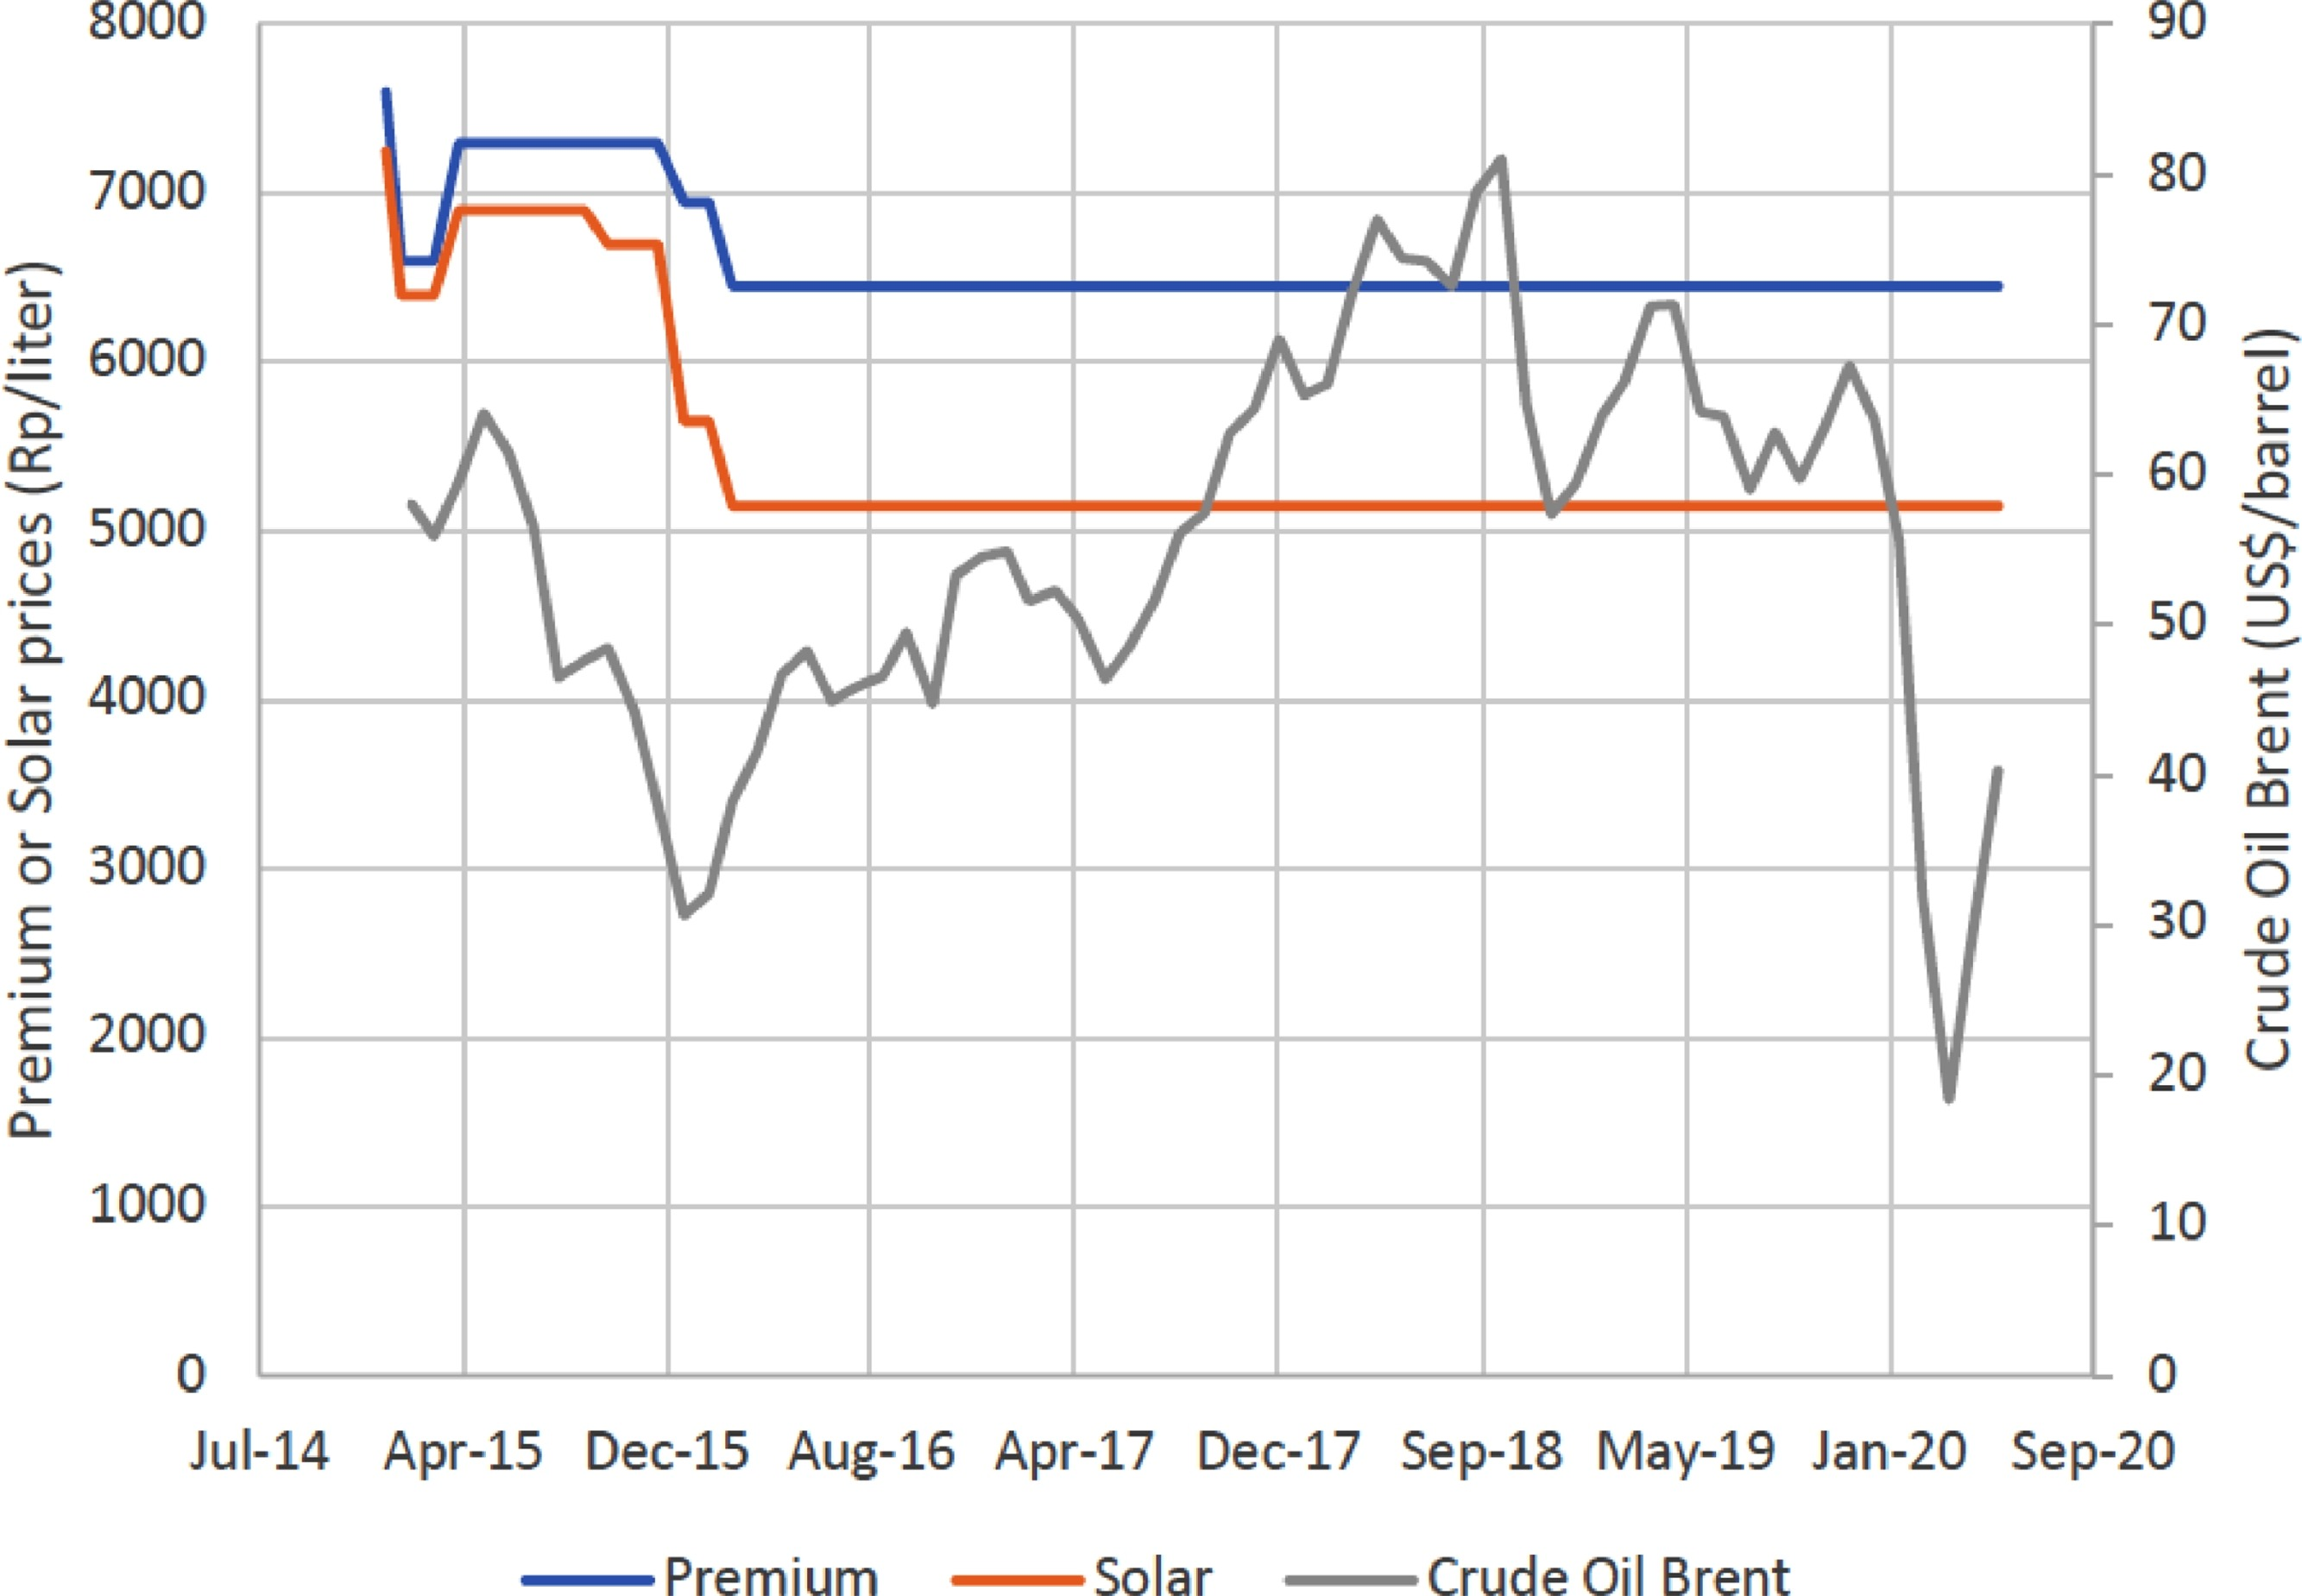
\includegraphics[scale=0.7]{Final_Project/image/bbm-price-2014-2018.jpg}
\caption{Subsidized Fuel Price at Government's Price Control 2014-2018}
\note{Source: \citet{ichsan_2022}}
\label{f:1}
\end{figure}


\begin{figure}[h]
\subcaptionbox{Village status in 2014\label{f:panel1}}{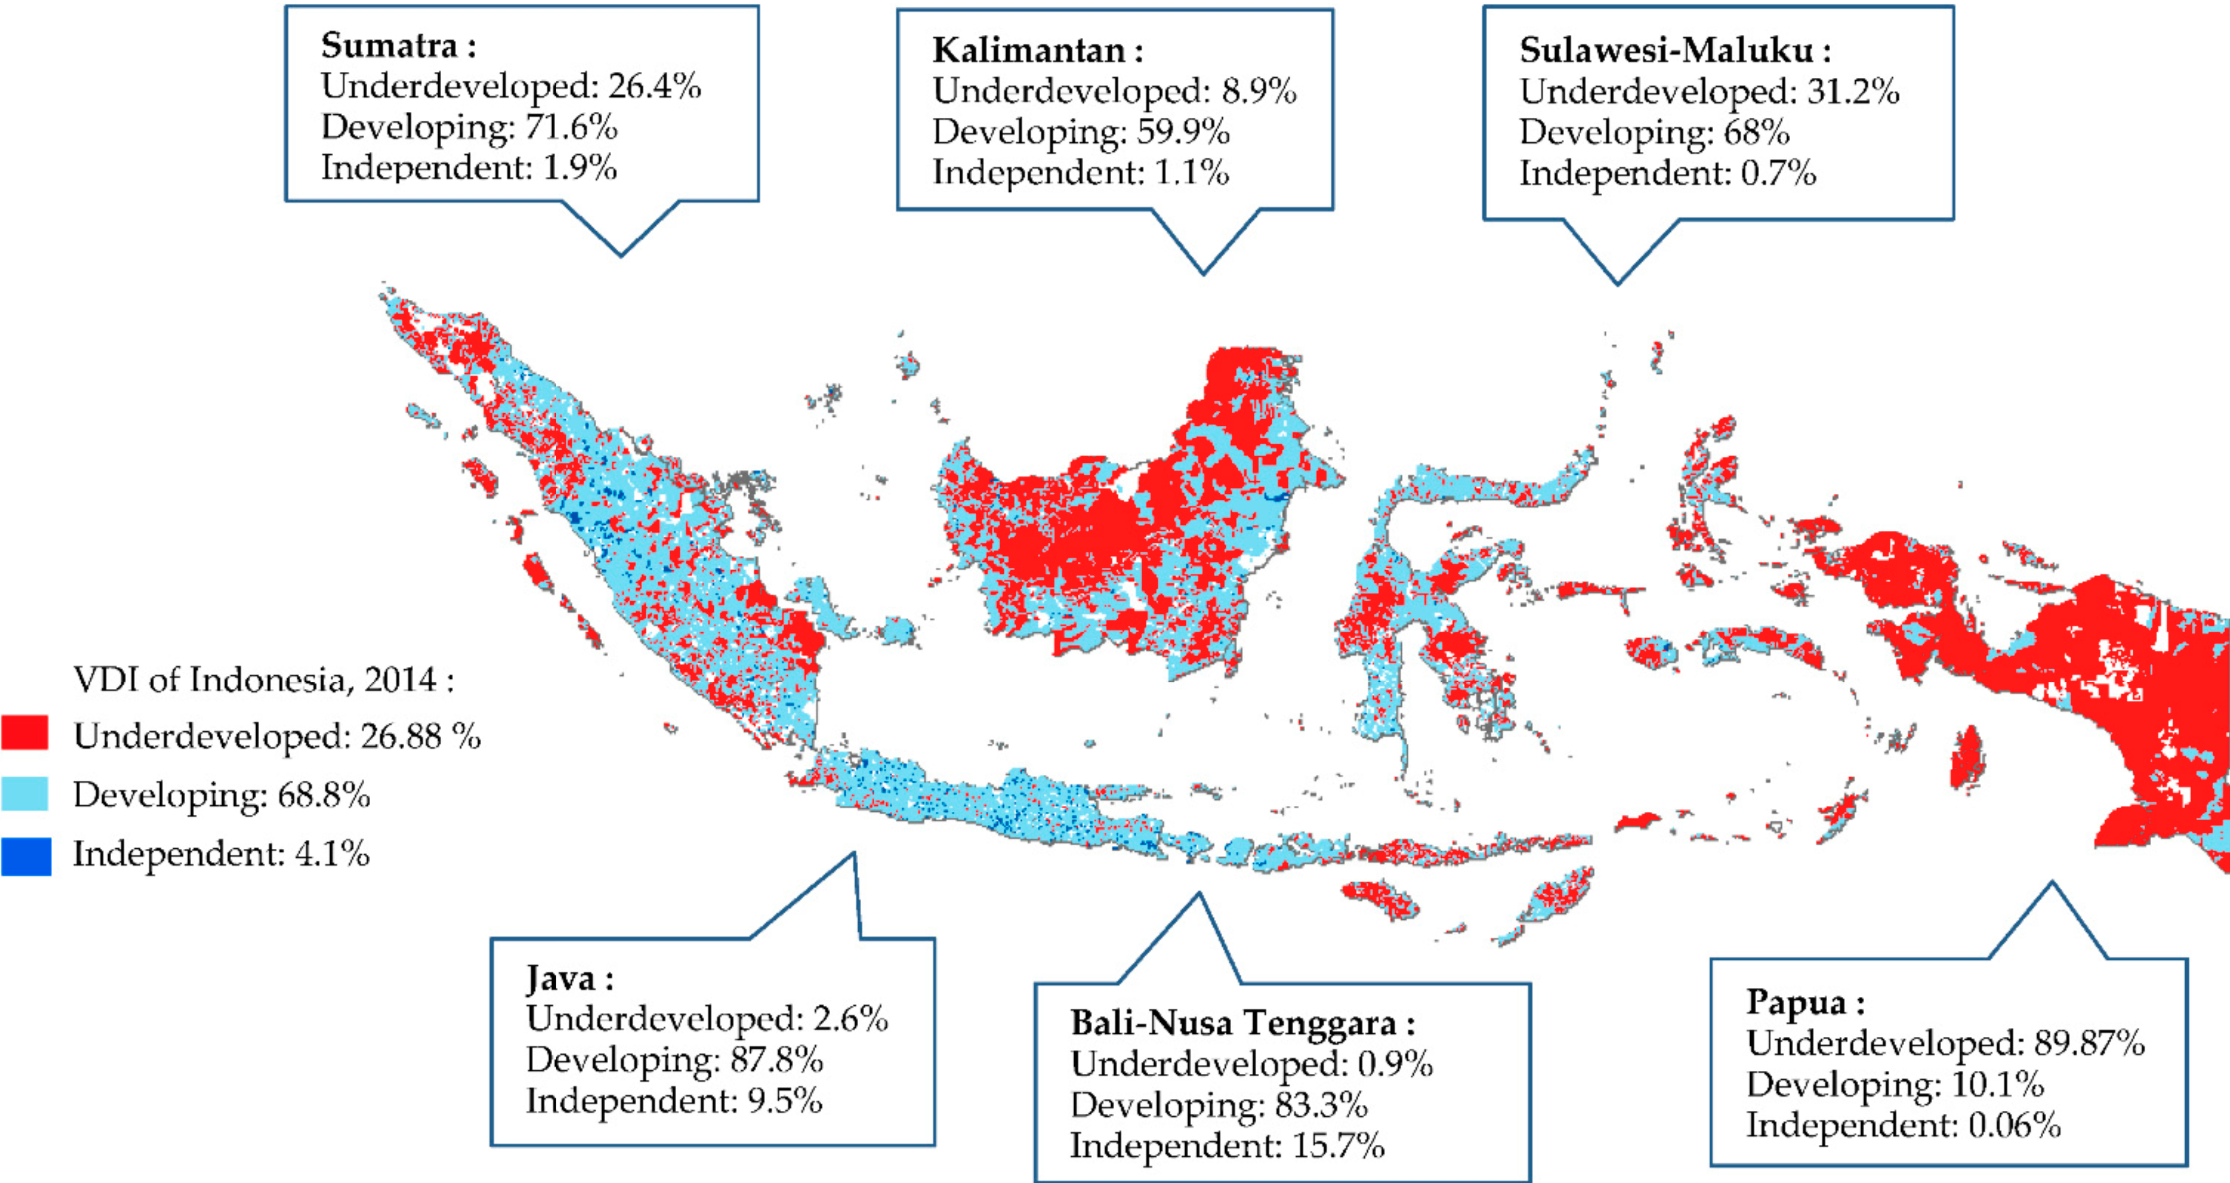
\includegraphics[scale=0.4]{Final_Project/image/vdi2014.png}}\hfill
\subcaptionbox{Village status in 2018\label{f:panel2}}{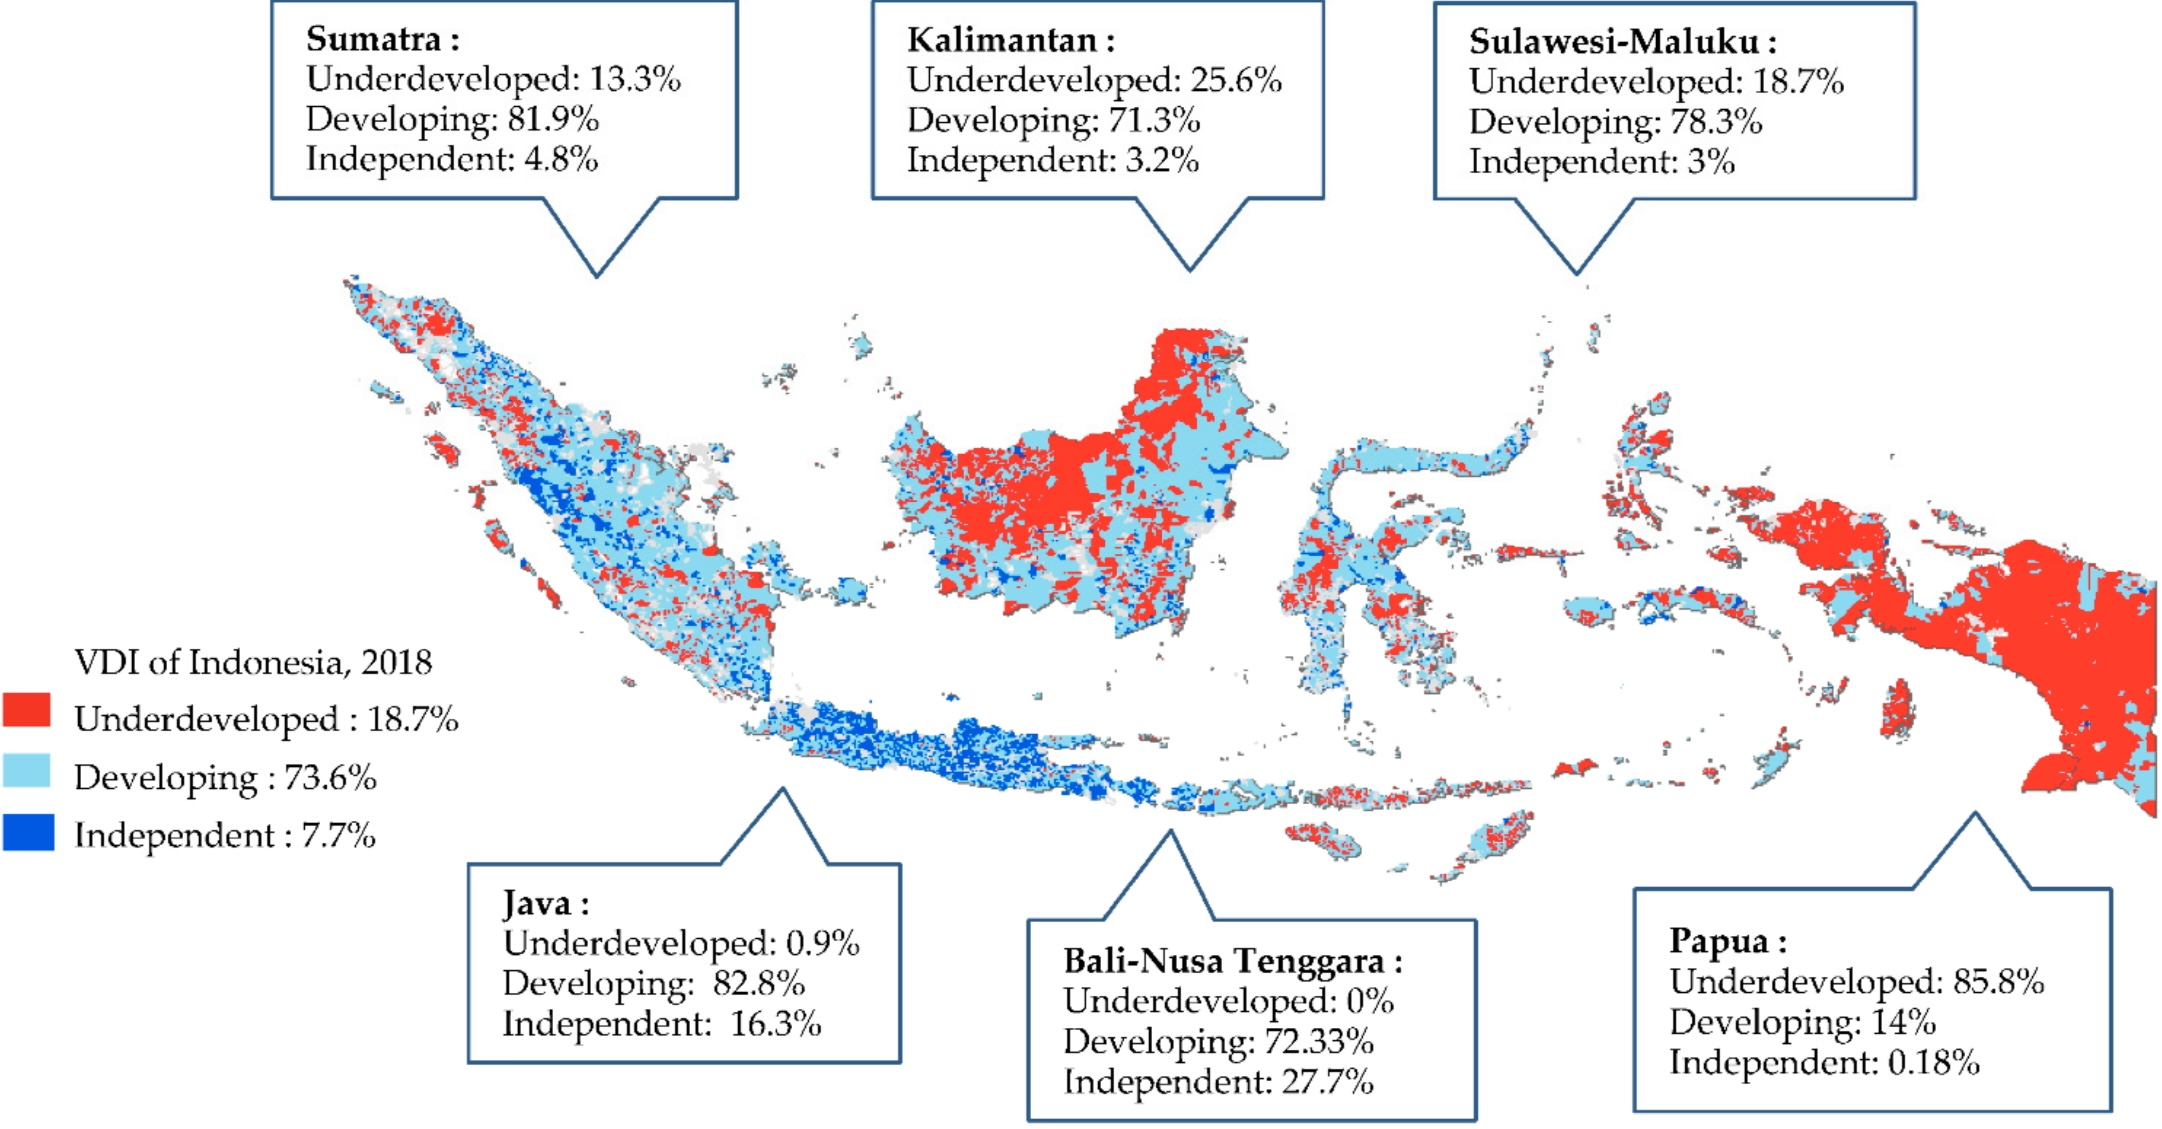
\includegraphics[scale=0.41]{Final_Project/image/vdi2018.jpg}}
\caption{Indonesia's Village Development Index status}
\note{Source: Statistics Indonesia from \citet{hartojo_2022}}
\label{f:2}\end{figure}

\begin{landscape}
\begin{figure}[t]
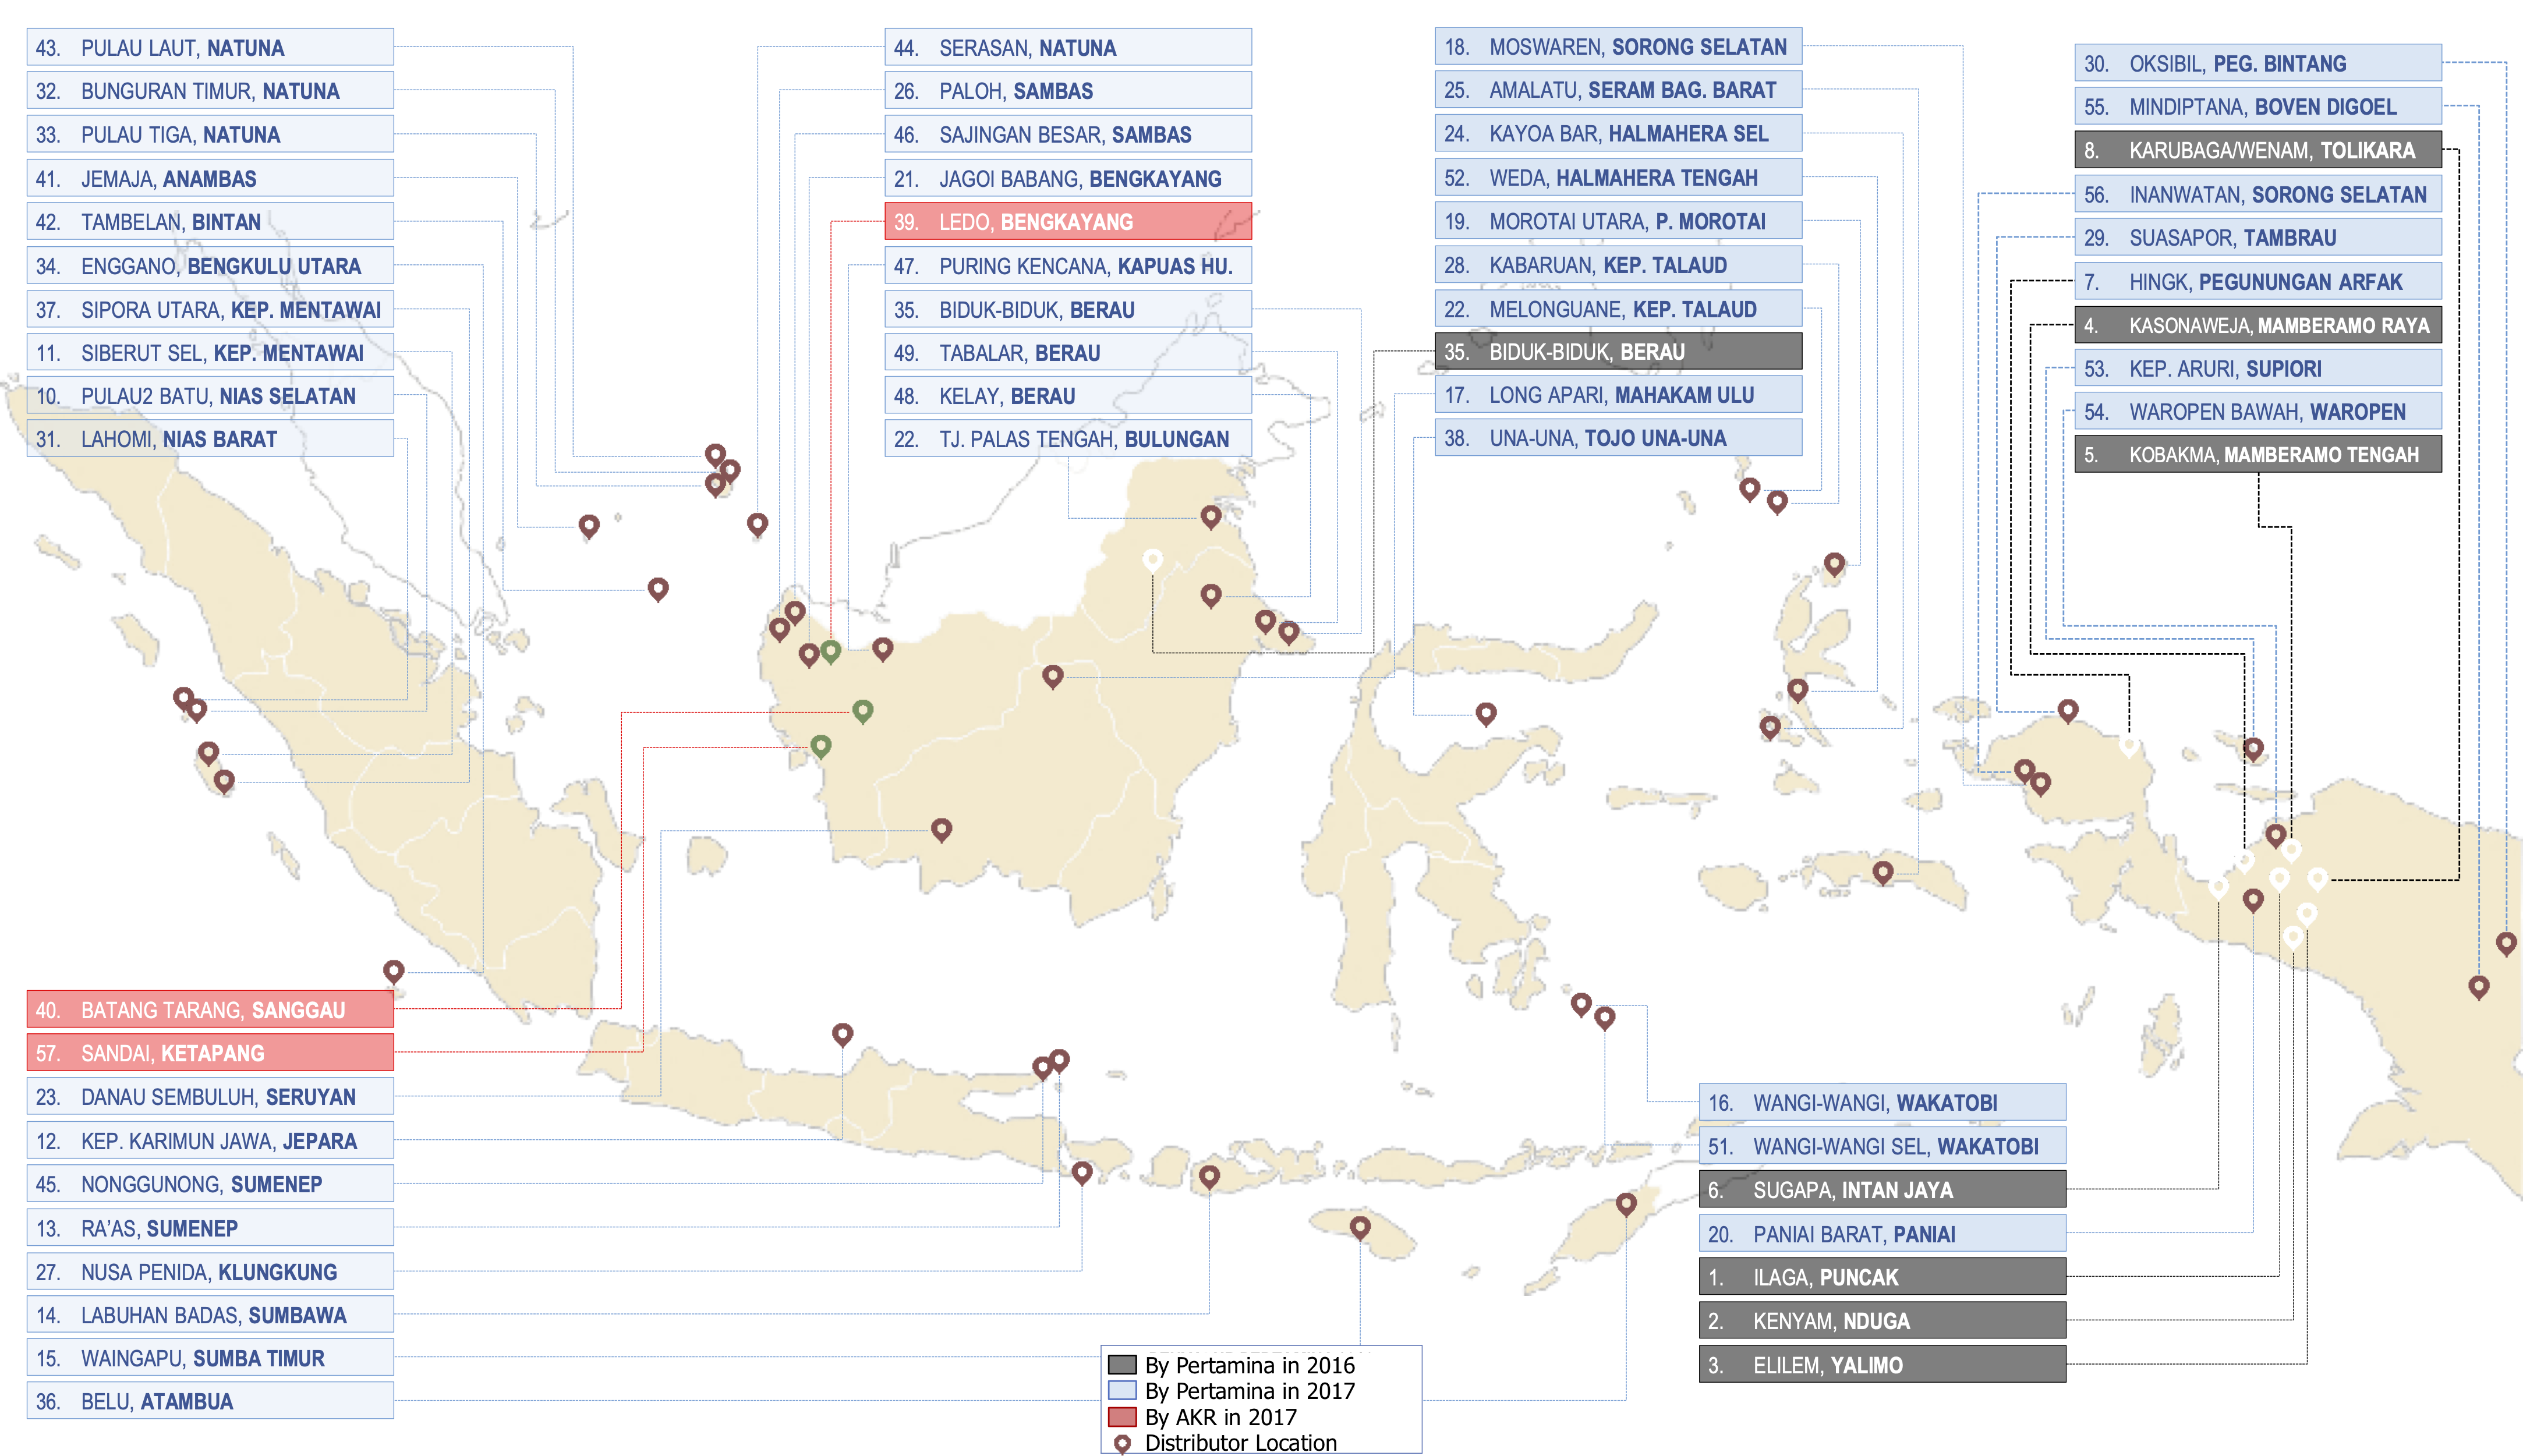
\includegraphics[scale=0.8]{Final_Project/image/BBM Satu Harga.png}
\caption{Location of the One Price Fuel Program in 2016-2017}
\label{f:3}
\end{figure}
\end{landscape}
 
\end{document}
